
    \documentclass{standalone}
    \usepackage{tikz}
    \usetikzlibrary{arrows, automata, positioning}
    \begin{document}
    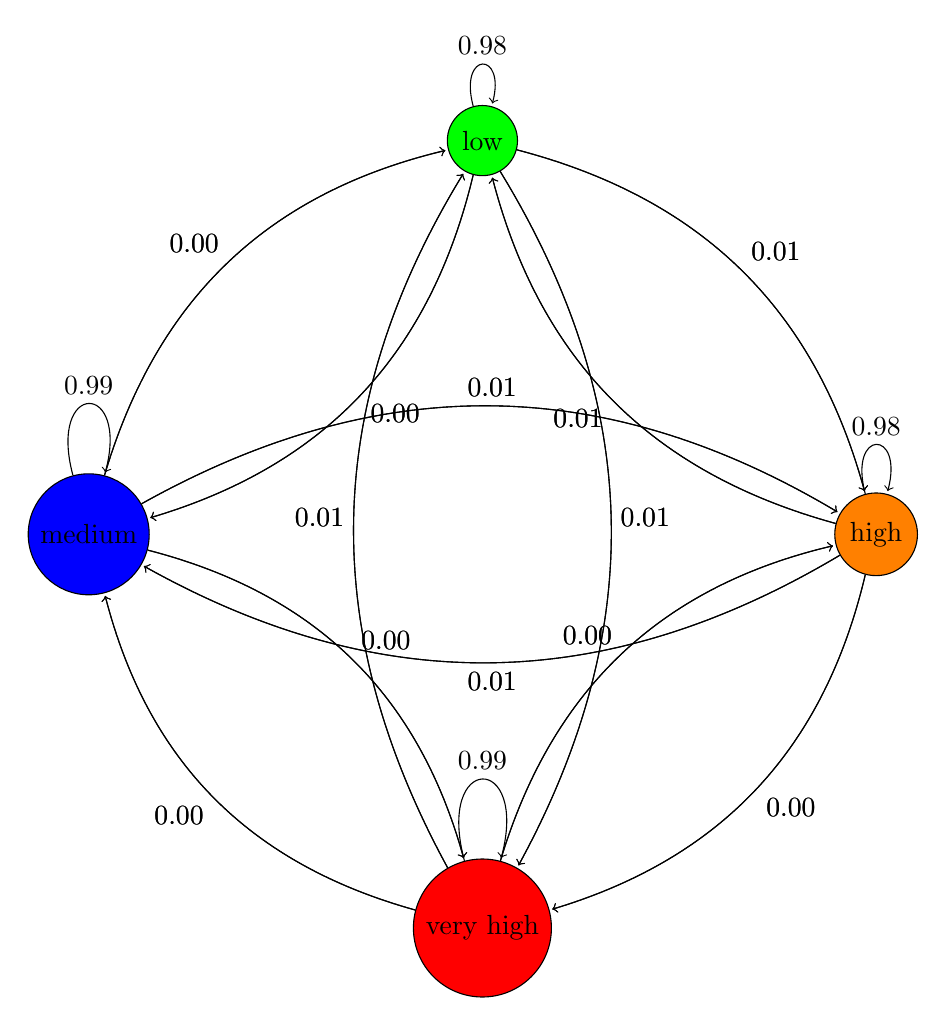
\begin{tikzpicture}[shorten >=1pt, node distance=4cm, on grid, auto]
    \node[state, fill=orange] (S0) at (5,0) {high} ;
\node[state, fill=green] (S1) at (0,5) {low} ;
\node[state, fill=blue] (S2) at (-5,0) {medium} ;
\node[state, fill=red] (S3) at (0,-5) {very high} ;
\path[->] (S0) edge [loop above] node {\(0.98\)} (S0);
\path[->] (S0) edge [bend left] node {\(0.01\)} (S1);
\path[->] (S1) edge [bend left] node {\(0.01\)} (S0);
\path[->] (S0) edge [bend left] node {\(0.01\)} (S2);
\path[->] (S2) edge [bend left] node {\(0.01\)} (S0);
\path[->] (S0) edge [bend left] node {\(0.00\)} (S3);
\path[->] (S3) edge [bend left] node {\(0.00\)} (S0);
\path[->] (S1) edge [bend left] node {\(0.01\)} (S0);
\path[->] (S0) edge [bend left] node {\(0.01\)} (S1);
\path[->] (S1) edge [loop above] node {\(0.98\)} (S1);
\path[->] (S1) edge [bend left] node {\(0.00\)} (S2);
\path[->] (S2) edge [bend left] node {\(0.00\)} (S1);
\path[->] (S1) edge [bend left] node {\(0.01\)} (S3);
\path[->] (S3) edge [bend left] node {\(0.01\)} (S1);
\path[->] (S2) edge [bend left] node {\(0.01\)} (S0);
\path[->] (S0) edge [bend left] node {\(0.01\)} (S2);
\path[->] (S2) edge [bend left] node {\(0.00\)} (S1);
\path[->] (S1) edge [bend left] node {\(0.00\)} (S2);
\path[->] (S2) edge [loop above] node {\(0.99\)} (S2);
\path[->] (S2) edge [bend left] node {\(0.00\)} (S3);
\path[->] (S3) edge [bend left] node {\(0.00\)} (S2);
\path[->] (S3) edge [bend left] node {\(0.00\)} (S0);
\path[->] (S0) edge [bend left] node {\(0.00\)} (S3);
\path[->] (S3) edge [bend left] node {\(0.01\)} (S1);
\path[->] (S1) edge [bend left] node {\(0.01\)} (S3);
\path[->] (S3) edge [bend left] node {\(0.00\)} (S2);
\path[->] (S2) edge [bend left] node {\(0.00\)} (S3);
\path[->] (S3) edge [loop above] node {\(0.99\)} (S3);

    \end{tikzpicture}
    \end{document}
    